\section{Results}

The data given by the user study allowed us to define 5 main types of interaction. Those interactions are defined by the way the user interacts with the plant. The 5 main types of interaction are :

\begin{itemize}
    \item Grasp : user uses the whole hand to grab trunk or leaves.
    \item Pinch : user uses 2 to 3 digits to grab trunk or leaves.
    \item Slide : user uses his/her hand or finger to slide on the plant whether is on a leave or on the trunk. The action is continuous.
    \item Pet : user uses his/her hand to cuddle the plant or to pass through the leaves. The user is moving his/her hand in space. She/he is not staying still or staying on a particular object.
    \item Tam Tam : user taps on the plant mainly using the whole hand.
\end{itemize}



Looking at the results, we extracted the table \ref{tab:results}.


\begin{table}[ht]
\begin{tabular}{|l|ll|l|ll|}
\hline
\multirow{2}{*}{Plant/Interaction} & \multicolumn{2}{l|}{Group 1}       & Group 2 & \multicolumn{2}{l|}{Group 3}       \\ \cline{2-6} 
                                   & \multicolumn{1}{l|}{Grasp} & Pinch & Slide   & \multicolumn{1}{l|}{Pet} & Tam Tam \\ \hline
Plant N°1                          & \multicolumn{1}{l|}{4}     & 8     & 4       & \multicolumn{1}{l|}{4}   & 2       \\ \hline
Plant N°2                          & \multicolumn{1}{l|}{9}     & 3     & 3       & \multicolumn{1}{l|}{3}   & 10      \\ \hline
Plant N°3                          & \multicolumn{1}{l|}{10}    & 1     & 5       & \multicolumn{1}{l|}{7}   & 3       \\ \hline
Total                              & \multicolumn{1}{l|}{23}    & 12    & 12      & \multicolumn{1}{l|}{14}  & 15      \\ \hline
\end{tabular}
% \caption*{Plant N°1 : Petite | Plant N°2 : Grande | Plant N°3 : Fougère}
\caption{Raw results extracted from the user study}
\label{tab:results}
\end{table}


\newpage

With the extraction of the result we were able to design a bar chart.
The graph is grouping the interactions by plant. The height of the bar is the number of participants that performed the interaction.
The graph is shown in figure \ref{fig:setup_user_study}.


\begin{figure}[ht]
    \centering
    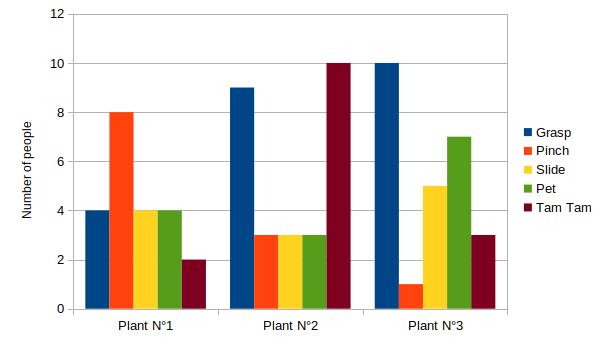
\includegraphics[width=0.42\textwidth]{Images/plant_interaction_chart_2.png}
    \caption{Bar chart that is extracting the main types of interaction regarding each plants.}
    
    \vspace{-0.5cm}
    \label{fig:setup_user_study}
    \vspace{0.2cm}
\end{figure}

In the end, of the 22 participants, 15 were already familiar with the project and 7 were not.



% \newpage

